\documentclass{article}
\usepackage{tikz}
\usepackage[margin=0.5in]{geometry}
\usetikzlibrary{trees}

\begin{document}

\begin{center}
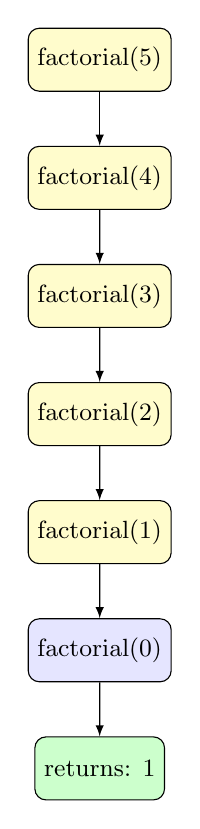
\begin{tikzpicture}[
  level distance=1.5cm,
  level 1/.style={sibling distance=4cm},
  level 2/.style={sibling distance=2cm},
  level 3/.style={sibling distance=1.5cm},
  every node/.style={rectangle, draw, rounded corners, 
                     fill=blue!10, align=center,
                     minimum height=0.8cm, font=\small},
  edge from parent/.style={draw, -latex},
  base/.style={fill=green!20},
  recursive/.style={fill=yellow!20}
]

\node[recursive] {factorial(5)}
    child {
        node[recursive] {factorial(4)}
            child {
                node[recursive] {factorial(3)}
                    child {
                        node[recursive] {factorial(2)}
                            child {
                                node[recursive] {factorial(1)}
                                    child {
                                        node {factorial(0)}
                                            child {node[base] {returns: 1}}
                                    }
                            }
                    }
            }
    }
;

\end{tikzpicture}
\end{center}

\vspace{1cm}

\textbf{Legend:}
\begin{itemize}
\item Blue nodes: Recursive calls
\item Green nodes: Base cases (leaf nodes)
\end{itemize}

\end{document}